\documentclass[twoside]{book}

% Packages required by doxygen
\usepackage{fixltx2e}
\usepackage{calc}
\usepackage{doxygen}
\usepackage[export]{adjustbox} % also loads graphicx
\usepackage{graphicx}
\usepackage[utf8]{inputenc}
\usepackage{makeidx}
\usepackage{multicol}
\usepackage{multirow}
\PassOptionsToPackage{warn}{textcomp}
\usepackage{textcomp}
\usepackage[nointegrals]{wasysym}
\usepackage[table]{xcolor}

% Font selection
\usepackage[T1]{fontenc}
\usepackage[scaled=.90]{helvet}
\usepackage{courier}
\usepackage{amssymb}
\usepackage{sectsty}
\renewcommand{\familydefault}{\sfdefault}
\allsectionsfont{%
  \fontseries{bc}\selectfont%
  \color{darkgray}%
}
\renewcommand{\DoxyLabelFont}{%
  \fontseries{bc}\selectfont%
  \color{darkgray}%
}
\newcommand{\+}{\discretionary{\mbox{\scriptsize$\hookleftarrow$}}{}{}}

% Page & text layout
\usepackage{geometry}
\geometry{%
  a4paper,%
  top=2.5cm,%
  bottom=2.5cm,%
  left=2.5cm,%
  right=2.5cm%
}
\tolerance=750
\hfuzz=15pt
\hbadness=750
\setlength{\emergencystretch}{15pt}
\setlength{\parindent}{0cm}
\setlength{\parskip}{3ex plus 2ex minus 2ex}
\makeatletter
\renewcommand{\paragraph}{%
  \@startsection{paragraph}{4}{0ex}{-1.0ex}{1.0ex}{%
    \normalfont\normalsize\bfseries\SS@parafont%
  }%
}
\renewcommand{\subparagraph}{%
  \@startsection{subparagraph}{5}{0ex}{-1.0ex}{1.0ex}{%
    \normalfont\normalsize\bfseries\SS@subparafont%
  }%
}
\makeatother

% Headers & footers
\usepackage{fancyhdr}
\pagestyle{fancyplain}
\fancyhead[LE]{\fancyplain{}{\bfseries\thepage}}
\fancyhead[CE]{\fancyplain{}{}}
\fancyhead[RE]{\fancyplain{}{\bfseries\leftmark}}
\fancyhead[LO]{\fancyplain{}{\bfseries\rightmark}}
\fancyhead[CO]{\fancyplain{}{}}
\fancyhead[RO]{\fancyplain{}{\bfseries\thepage}}
\fancyfoot[LE]{\fancyplain{}{}}
\fancyfoot[CE]{\fancyplain{}{}}
\fancyfoot[RE]{\fancyplain{}{\bfseries\scriptsize Generated by Doxygen }}
\fancyfoot[LO]{\fancyplain{}{\bfseries\scriptsize Generated by Doxygen }}
\fancyfoot[CO]{\fancyplain{}{}}
\fancyfoot[RO]{\fancyplain{}{}}
\renewcommand{\footrulewidth}{0.4pt}
\renewcommand{\chaptermark}[1]{%
  \markboth{#1}{}%
}
\renewcommand{\sectionmark}[1]{%
  \markright{\thesection\ #1}%
}

% Indices & bibliography
\usepackage{natbib}
\usepackage[titles]{tocloft}
\setcounter{tocdepth}{3}
\setcounter{secnumdepth}{5}
\makeindex

% Hyperlinks (required, but should be loaded last)
\usepackage{ifpdf}
\ifpdf
  \usepackage[pdftex,pagebackref=true]{hyperref}
\else
  \usepackage[ps2pdf,pagebackref=true]{hyperref}
\fi
\hypersetup{%
  colorlinks=true,%
  linkcolor=blue,%
  citecolor=blue,%
  unicode%
}

% Custom commands
\newcommand{\clearemptydoublepage}{%
  \newpage{\pagestyle{empty}\cleardoublepage}%
}

\usepackage{caption}
\captionsetup{labelsep=space,justification=centering,font={bf},singlelinecheck=off,skip=4pt,position=top}

%===== C O N T E N T S =====

\begin{document}

% Titlepage & ToC
\hypersetup{pageanchor=false,
             bookmarksnumbered=true,
             pdfencoding=unicode
            }
\pagenumbering{roman}
\begin{titlepage}
\vspace*{7cm}
\begin{center}%
{\Large lab8 }\\
\vspace*{1cm}
{\large Generated by Doxygen 1.8.11}\\
\end{center}
\end{titlepage}
\clearemptydoublepage
\tableofcontents
\clearemptydoublepage
\pagenumbering{arabic}
\hypersetup{pageanchor=true}

%--- Begin generated contents ---
\chapter{Class Index}
\section{Class List}
Here are the classes, structs, unions and interfaces with brief descriptions\+:\begin{DoxyCompactList}
\item\contentsline{section}{\hyperlink{classActor}{Actor} \\*Defines a favorite \hyperlink{classActor}{Actor} }{\pageref{classActor}}{}
\item\contentsline{section}{\hyperlink{classRequest}{Request} \\*Defines a client request }{\pageref{classRequest}}{}
\item\contentsline{section}{\hyperlink{classResponse}{Response} \\*Defines a server response }{\pageref{classResponse}}{}
\end{DoxyCompactList}

\chapter{File Index}
\section{File List}
Here is a list of all documented files with brief descriptions\+:\begin{DoxyCompactList}
\item\contentsline{section}{include/\hyperlink{actor_8h}{actor.\+h} \\*Data about favorite \hyperlink{classActor}{Actor} }{\pageref{actor_8h}}{}
\item\contentsline{section}{include/\hyperlink{parserJson_8h}{parser\+Json.\+h} \\*Module to parse data to Json string }{\pageref{parserJson_8h}}{}
\item\contentsline{section}{include/\hyperlink{request_8h}{request.\+h} \\*Wrapper for client request }{\pageref{request_8h}}{}
\item\contentsline{section}{include/\hyperlink{response_8h}{response.\+h} \\*Wrapper for server response }{\pageref{response_8h}}{}
\end{DoxyCompactList}

\chapter{Class Documentation}
\hypertarget{classActor}{}\section{Actor Class Reference}
\label{classActor}\index{Actor@{Actor}}


defines a favorite \hyperlink{classActor}{Actor}  




{\ttfamily \#include $<$actor.\+h$>$}

\subsection*{Public Member Functions}
\begin{DoxyCompactItemize}
\item 
\hyperlink{classActor_a2a0ff4335a1ee9096df90f288c026c8b}{Actor} ()\hypertarget{classActor_a2a0ff4335a1ee9096df90f288c026c8b}{}\label{classActor_a2a0ff4335a1ee9096df90f288c026c8b}

\begin{DoxyCompactList}\small\item\em default public constructor for \hyperlink{classActor}{Actor} \end{DoxyCompactList}\item 
\hyperlink{classActor_ad807fe8f85e72ab263a0c05e3231cb39}{$\sim$\+Actor} ()\hypertarget{classActor_ad807fe8f85e72ab263a0c05e3231cb39}{}\label{classActor_ad807fe8f85e72ab263a0c05e3231cb39}

\begin{DoxyCompactList}\small\item\em default public destructor for \hyperlink{classActor}{Actor} \end{DoxyCompactList}\item 
\hyperlink{classActor_ab6b4c8694911ae124e16b03506570a2f}{Actor} (int \hyperlink{classActor_a6da7fe13f5cee31d8d68ef04fb173fed}{id}, string \hyperlink{classActor_a28da8d9137bc756d0a878081f2f87e75}{name}, string \hyperlink{classActor_a10673442999877b7fa58b44e89867ec8}{nation}, int \hyperlink{classActor_a1b075c42ebb2a88e76c43dbb8de279db}{age})
\begin{DoxyCompactList}\small\item\em public constructor for \hyperlink{classActor}{Actor} that fill all fields in \hyperlink{classActor}{Actor} \end{DoxyCompactList}\item 
int \hyperlink{classActor_a6da7fe13f5cee31d8d68ef04fb173fed}{id} ()
\begin{DoxyCompactList}\small\item\em get id of \hyperlink{classActor}{Actor} \end{DoxyCompactList}\item 
string \hyperlink{classActor_a28da8d9137bc756d0a878081f2f87e75}{name} ()
\begin{DoxyCompactList}\small\item\em get name of \hyperlink{classActor}{Actor} \end{DoxyCompactList}\item 
string \hyperlink{classActor_a10673442999877b7fa58b44e89867ec8}{nation} ()
\begin{DoxyCompactList}\small\item\em get nation of \hyperlink{classActor}{Actor} \end{DoxyCompactList}\item 
int \hyperlink{classActor_a1b075c42ebb2a88e76c43dbb8de279db}{age} ()
\begin{DoxyCompactList}\small\item\em get age of \hyperlink{classActor}{Actor} \end{DoxyCompactList}\item 
string \hyperlink{classActor_a208ca77aceb8e6ac7f8a76b7ad1eb719}{value\+By\+Field} (string field)
\begin{DoxyCompactList}\small\item\em get value that contain specified filed of \hyperlink{classActor}{Actor} \end{DoxyCompactList}\end{DoxyCompactItemize}


\subsection{Detailed Description}
defines a favorite \hyperlink{classActor}{Actor} 

\subsection{Constructor \& Destructor Documentation}
\index{Actor@{Actor}!Actor@{Actor}}
\index{Actor@{Actor}!Actor@{Actor}}
\subsubsection[{\texorpdfstring{Actor(int id, string name, string nation, int age)}{Actor(int id, string name, string nation, int age)}}]{\setlength{\rightskip}{0pt plus 5cm}Actor\+::\+Actor (
\begin{DoxyParamCaption}
\item[{int}]{id, }
\item[{string}]{name, }
\item[{string}]{nation, }
\item[{int}]{age}
\end{DoxyParamCaption}
)}\hypertarget{classActor_ab6b4c8694911ae124e16b03506570a2f}{}\label{classActor_ab6b4c8694911ae124e16b03506570a2f}


public constructor for \hyperlink{classActor}{Actor} that fill all fields in \hyperlink{classActor}{Actor} 


\begin{DoxyParams}{Parameters}
{\em id} & -\/ unique number of \hyperlink{classActor}{Actor} \\
\hline
{\em name} & -\/ name of \hyperlink{classActor}{Actor} \\
\hline
{\em nation} & -\/ nationality of \hyperlink{classActor}{Actor} \\
\hline
{\em age} & -\/ \hyperlink{classActor}{Actor}\textquotesingle{}s age \\
\hline
\end{DoxyParams}


\subsection{Member Function Documentation}
\index{Actor@{Actor}!age@{age}}
\index{age@{age}!Actor@{Actor}}
\subsubsection[{\texorpdfstring{age()}{age()}}]{\setlength{\rightskip}{0pt plus 5cm}int Actor\+::age (
\begin{DoxyParamCaption}
{}
\end{DoxyParamCaption}
)}\hypertarget{classActor_a1b075c42ebb2a88e76c43dbb8de279db}{}\label{classActor_a1b075c42ebb2a88e76c43dbb8de279db}


get age of \hyperlink{classActor}{Actor} 

\begin{DoxyReturn}{Returns}
string that represents age of \hyperlink{classActor}{Actor} 
\end{DoxyReturn}
\index{Actor@{Actor}!id@{id}}
\index{id@{id}!Actor@{Actor}}
\subsubsection[{\texorpdfstring{id()}{id()}}]{\setlength{\rightskip}{0pt plus 5cm}int Actor\+::id (
\begin{DoxyParamCaption}
{}
\end{DoxyParamCaption}
)}\hypertarget{classActor_a6da7fe13f5cee31d8d68ef04fb173fed}{}\label{classActor_a6da7fe13f5cee31d8d68ef04fb173fed}


get id of \hyperlink{classActor}{Actor} 

\begin{DoxyReturn}{Returns}
string that represents unique number of \hyperlink{classActor}{Actor} 
\end{DoxyReturn}
\index{Actor@{Actor}!name@{name}}
\index{name@{name}!Actor@{Actor}}
\subsubsection[{\texorpdfstring{name()}{name()}}]{\setlength{\rightskip}{0pt plus 5cm}string Actor\+::name (
\begin{DoxyParamCaption}
{}
\end{DoxyParamCaption}
)}\hypertarget{classActor_a28da8d9137bc756d0a878081f2f87e75}{}\label{classActor_a28da8d9137bc756d0a878081f2f87e75}


get name of \hyperlink{classActor}{Actor} 

\begin{DoxyReturn}{Returns}
string that represents name of \hyperlink{classActor}{Actor} 
\end{DoxyReturn}
\index{Actor@{Actor}!nation@{nation}}
\index{nation@{nation}!Actor@{Actor}}
\subsubsection[{\texorpdfstring{nation()}{nation()}}]{\setlength{\rightskip}{0pt plus 5cm}string Actor\+::nation (
\begin{DoxyParamCaption}
{}
\end{DoxyParamCaption}
)}\hypertarget{classActor_a10673442999877b7fa58b44e89867ec8}{}\label{classActor_a10673442999877b7fa58b44e89867ec8}


get nation of \hyperlink{classActor}{Actor} 

\begin{DoxyReturn}{Returns}
string that represents nationality of \hyperlink{classActor}{Actor} 
\end{DoxyReturn}
\index{Actor@{Actor}!value\+By\+Field@{value\+By\+Field}}
\index{value\+By\+Field@{value\+By\+Field}!Actor@{Actor}}
\subsubsection[{\texorpdfstring{value\+By\+Field(string field)}{valueByField(string field)}}]{\setlength{\rightskip}{0pt plus 5cm}string Actor\+::value\+By\+Field (
\begin{DoxyParamCaption}
\item[{string}]{field}
\end{DoxyParamCaption}
)}\hypertarget{classActor_a208ca77aceb8e6ac7f8a76b7ad1eb719}{}\label{classActor_a208ca77aceb8e6ac7f8a76b7ad1eb719}


get value that contain specified filed of \hyperlink{classActor}{Actor} 


\begin{DoxyParams}{Parameters}
{\em field} & -\/ string that defines field which value returns \\
\hline
\end{DoxyParams}
\begin{DoxyReturn}{Returns}
string that represents value at specified field 
\end{DoxyReturn}


The documentation for this class was generated from the following files\+:\begin{DoxyCompactItemize}
\item 
include/\hyperlink{actor_8h}{actor.\+h}\item 
src/actor.\+cpp\end{DoxyCompactItemize}

\hypertarget{classRequest}{}\section{Request Class Reference}
\label{classRequest}\index{Request@{Request}}


defines a client request  




{\ttfamily \#include $<$request.\+h$>$}

\subsection*{Public Member Functions}
\begin{DoxyCompactItemize}
\item 
\hyperlink{classRequest_afaf8d8928de7ffff8a3767589489bd33}{Request} ()\hypertarget{classRequest_afaf8d8928de7ffff8a3767589489bd33}{}\label{classRequest_afaf8d8928de7ffff8a3767589489bd33}

\begin{DoxyCompactList}\small\item\em default public constructor for \hyperlink{classRequest}{Request} \end{DoxyCompactList}\item 
\hyperlink{classRequest_a3b25fd1c24befd84e55ec36d012dfd29}{Request} (string request)
\begin{DoxyCompactList}\small\item\em public constructor for \hyperlink{classRequest}{Request} that process string as request \end{DoxyCompactList}\item 
\hyperlink{classRequest_a4d57c725686701f773eb3630630a7ea2}{$\sim$\+Request} ()\hypertarget{classRequest_a4d57c725686701f773eb3630630a7ea2}{}\label{classRequest_a4d57c725686701f773eb3630630a7ea2}

\begin{DoxyCompactList}\small\item\em default public destructor for \hyperlink{classRequest}{Request} \end{DoxyCompactList}\item 
string \hyperlink{classRequest_a8cc222c2c9b1f27b0805401a9c657789}{method} ()
\begin{DoxyCompactList}\small\item\em get method from client \hyperlink{classRequest}{Request} \end{DoxyCompactList}\item 
string \hyperlink{classRequest_ac2b4080268fb8f61e74d96f30f1b1b95}{path} ()
\begin{DoxyCompactList}\small\item\em get path from client \hyperlink{classRequest}{Request} \end{DoxyCompactList}\item 
string \hyperlink{classRequest_a0065bb0a4c9fe961cb7f9386e15d0fed}{key} ()
\begin{DoxyCompactList}\small\item\em get specified key in path from client \hyperlink{classRequest}{Request} \end{DoxyCompactList}\item 
string \hyperlink{classRequest_a5d98408923e7921454b321b2c6e64471}{value} ()
\begin{DoxyCompactList}\small\item\em get specified value in path from client \hyperlink{classRequest}{Request} \end{DoxyCompactList}\end{DoxyCompactItemize}


\subsection{Detailed Description}
defines a client request 

\subsection{Constructor \& Destructor Documentation}
\index{Request@{Request}!Request@{Request}}
\index{Request@{Request}!Request@{Request}}
\subsubsection[{\texorpdfstring{Request(string request)}{Request(string request)}}]{\setlength{\rightskip}{0pt plus 5cm}Request\+::\+Request (
\begin{DoxyParamCaption}
\item[{string}]{request}
\end{DoxyParamCaption}
)}\hypertarget{classRequest_a3b25fd1c24befd84e55ec36d012dfd29}{}\label{classRequest_a3b25fd1c24befd84e55ec36d012dfd29}


public constructor for \hyperlink{classRequest}{Request} that process string as request 


\begin{DoxyParams}{Parameters}
{\em request} & -\/ string for processing request \\
\hline
\end{DoxyParams}


\subsection{Member Function Documentation}
\index{Request@{Request}!key@{key}}
\index{key@{key}!Request@{Request}}
\subsubsection[{\texorpdfstring{key()}{key()}}]{\setlength{\rightskip}{0pt plus 5cm}string Request\+::key (
\begin{DoxyParamCaption}
{}
\end{DoxyParamCaption}
)}\hypertarget{classRequest_a0065bb0a4c9fe961cb7f9386e15d0fed}{}\label{classRequest_a0065bb0a4c9fe961cb7f9386e15d0fed}


get specified key in path from client \hyperlink{classRequest}{Request} 

\begin{DoxyReturn}{Returns}
string that defines specified key in path of \hyperlink{classRequest}{Request} 
\end{DoxyReturn}
\index{Request@{Request}!method@{method}}
\index{method@{method}!Request@{Request}}
\subsubsection[{\texorpdfstring{method()}{method()}}]{\setlength{\rightskip}{0pt plus 5cm}string Request\+::method (
\begin{DoxyParamCaption}
{}
\end{DoxyParamCaption}
)}\hypertarget{classRequest_a8cc222c2c9b1f27b0805401a9c657789}{}\label{classRequest_a8cc222c2c9b1f27b0805401a9c657789}


get method from client \hyperlink{classRequest}{Request} 

\begin{DoxyReturn}{Returns}
string that defines method of \hyperlink{classRequest}{Request} 
\end{DoxyReturn}
\index{Request@{Request}!path@{path}}
\index{path@{path}!Request@{Request}}
\subsubsection[{\texorpdfstring{path()}{path()}}]{\setlength{\rightskip}{0pt plus 5cm}string Request\+::path (
\begin{DoxyParamCaption}
{}
\end{DoxyParamCaption}
)}\hypertarget{classRequest_ac2b4080268fb8f61e74d96f30f1b1b95}{}\label{classRequest_ac2b4080268fb8f61e74d96f30f1b1b95}


get path from client \hyperlink{classRequest}{Request} 

\begin{DoxyReturn}{Returns}
string that defines path of \hyperlink{classRequest}{Request} 
\end{DoxyReturn}
\index{Request@{Request}!value@{value}}
\index{value@{value}!Request@{Request}}
\subsubsection[{\texorpdfstring{value()}{value()}}]{\setlength{\rightskip}{0pt plus 5cm}string Request\+::value (
\begin{DoxyParamCaption}
{}
\end{DoxyParamCaption}
)}\hypertarget{classRequest_a5d98408923e7921454b321b2c6e64471}{}\label{classRequest_a5d98408923e7921454b321b2c6e64471}


get specified value in path from client \hyperlink{classRequest}{Request} 

\begin{DoxyReturn}{Returns}
string that defines specified value in path of \hyperlink{classRequest}{Request} 
\end{DoxyReturn}


The documentation for this class was generated from the following files\+:\begin{DoxyCompactItemize}
\item 
include/\hyperlink{request_8h}{request.\+h}\item 
src/request.\+cpp\end{DoxyCompactItemize}

\hypertarget{classResponse}{}\section{Response Class Reference}
\label{classResponse}\index{Response@{Response}}


defines a server response  




{\ttfamily \#include $<$response.\+h$>$}

\subsection*{Public Member Functions}
\begin{DoxyCompactItemize}
\item 
\hyperlink{classResponse_aa9b6e391d77fce8daca8bac13730ec8e}{Response} ()\hypertarget{classResponse_aa9b6e391d77fce8daca8bac13730ec8e}{}\label{classResponse_aa9b6e391d77fce8daca8bac13730ec8e}

\begin{DoxyCompactList}\small\item\em default public constructor for \hyperlink{classResponse}{Response} \end{DoxyCompactList}\item 
\hyperlink{classResponse_a63ee2ba4663e70dfe54a9e6589a68e2a}{Response} (\hyperlink{classRequest}{Request} $\ast$request, vector$<$ \hyperlink{classActor}{Actor} $\ast$ $>$ Actors)
\begin{DoxyCompactList}\small\item\em public constructor for \hyperlink{classResponse}{Response} that process vector of Actors according to request \end{DoxyCompactList}\item 
\hyperlink{classResponse_a2a4a6403aaefce73725f17cf63896f84}{$\sim$\+Response} ()\hypertarget{classResponse_a2a4a6403aaefce73725f17cf63896f84}{}\label{classResponse_a2a4a6403aaefce73725f17cf63896f84}

\begin{DoxyCompactList}\small\item\em default public destructor for \hyperlink{classResponse}{Response} \end{DoxyCompactList}\item 
string \hyperlink{classResponse_a517690400a7b7091d03e917f335f7f28}{message} ()
\begin{DoxyCompactList}\small\item\em get message from \hyperlink{classResponse}{Response} \end{DoxyCompactList}\end{DoxyCompactItemize}


\subsection{Detailed Description}
defines a server response 

\subsection{Constructor \& Destructor Documentation}
\index{Response@{Response}!Response@{Response}}
\index{Response@{Response}!Response@{Response}}
\subsubsection[{\texorpdfstring{Response(\+Request $\ast$request, vector$<$ Actor $\ast$ $>$ Actors)}{Response(Request *request, vector< Actor * > Actors)}}]{\setlength{\rightskip}{0pt plus 5cm}Response\+::\+Response (
\begin{DoxyParamCaption}
\item[{{\bf Request} $\ast$}]{request, }
\item[{vector$<$ {\bf Actor} $\ast$ $>$}]{Actors}
\end{DoxyParamCaption}
)}\hypertarget{classResponse_a63ee2ba4663e70dfe54a9e6589a68e2a}{}\label{classResponse_a63ee2ba4663e70dfe54a9e6589a68e2a}


public constructor for \hyperlink{classResponse}{Response} that process vector of Actors according to request 


\begin{DoxyParams}{Parameters}
{\em request} & -\/ \hyperlink{classRequest}{Request} from client to process data \\
\hline
{\em vector} & of Actors that processed according to request \\
\hline
\end{DoxyParams}


\subsection{Member Function Documentation}
\index{Response@{Response}!message@{message}}
\index{message@{message}!Response@{Response}}
\subsubsection[{\texorpdfstring{message()}{message()}}]{\setlength{\rightskip}{0pt plus 5cm}string Response\+::message (
\begin{DoxyParamCaption}
{}
\end{DoxyParamCaption}
)}\hypertarget{classResponse_a517690400a7b7091d03e917f335f7f28}{}\label{classResponse_a517690400a7b7091d03e917f335f7f28}


get message from \hyperlink{classResponse}{Response} 

\begin{DoxyReturn}{Returns}
message that contained in \hyperlink{classResponse}{Response} 
\end{DoxyReturn}


The documentation for this class was generated from the following files\+:\begin{DoxyCompactItemize}
\item 
include/\hyperlink{response_8h}{response.\+h}\item 
src/response.\+cpp\end{DoxyCompactItemize}

\chapter{File Documentation}
\hypertarget{actor_8h}{}\section{include/actor.h File Reference}
\label{actor_8h}\index{include/actor.\+h@{include/actor.\+h}}


Data about favorite \hyperlink{classActor}{Actor}.  


{\ttfamily \#include $<$iostream$>$}\\*
Include dependency graph for actor.\+h\+:
\nopagebreak
\begin{figure}[H]
\begin{center}
\leavevmode
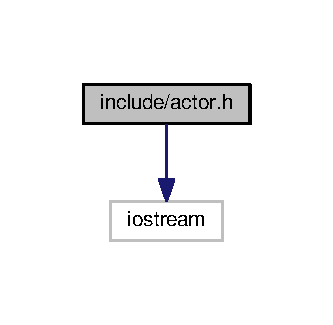
\includegraphics[width=160pt]{actor_8h__incl}
\end{center}
\end{figure}
This graph shows which files directly or indirectly include this file\+:
\nopagebreak
\begin{figure}[H]
\begin{center}
\leavevmode
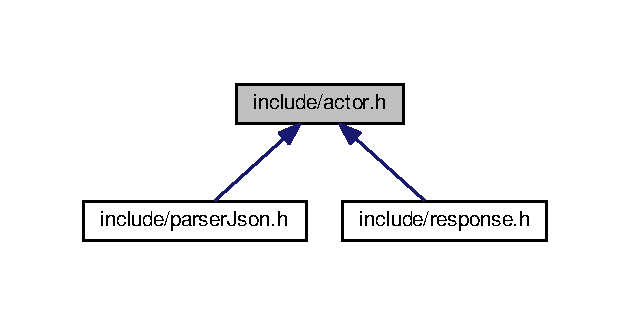
\includegraphics[width=303pt]{actor_8h__dep__incl}
\end{center}
\end{figure}
\subsection*{Classes}
\begin{DoxyCompactItemize}
\item 
class \hyperlink{classActor}{Actor}
\begin{DoxyCompactList}\small\item\em defines a favorite \hyperlink{classActor}{Actor} \end{DoxyCompactList}\end{DoxyCompactItemize}


\subsection{Detailed Description}
Data about favorite \hyperlink{classActor}{Actor}. 


\hypertarget{parserJson_8h}{}\section{include/parser\+Json.h File Reference}
\label{parserJson_8h}\index{include/parser\+Json.\+h@{include/parser\+Json.\+h}}


Module to parse data to Json string.  


{\ttfamily \#include $<$iostream$>$}\\*
{\ttfamily \#include $<$vector$>$}\\*
{\ttfamily \#include $<$actor.\+h$>$}\\*
Include dependency graph for parser\+Json.\+h\+:
\nopagebreak
\begin{figure}[H]
\begin{center}
\leavevmode
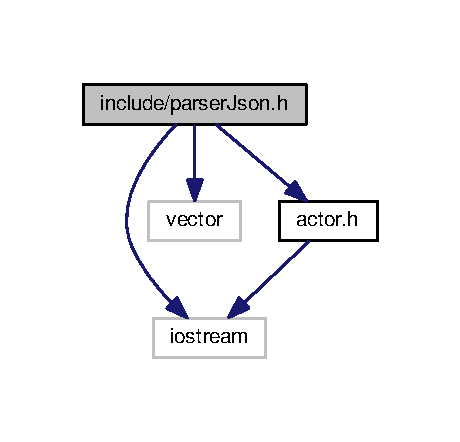
\includegraphics[width=221pt]{parserJson_8h__incl}
\end{center}
\end{figure}
\subsection*{Functions}
\begin{DoxyCompactItemize}
\item 
string \hyperlink{parserJson_8h_a4c799be6272b52be845ca68594a679fb}{parse\+Server\+Info} (void)
\begin{DoxyCompactList}\small\item\em get server information \end{DoxyCompactList}\item 
string \hyperlink{parserJson_8h_a812bf352d4eda2bca6cab059023d800d}{parse\+Actors} (vector$<$ \hyperlink{classActor}{Actor} $\ast$ $>$ Actors)
\begin{DoxyCompactList}\small\item\em get all Actors in Json fromat \end{DoxyCompactList}\item 
string \hyperlink{parserJson_8h_a2f09e2fb6c937c326ee0a32c5ba949b3}{parse\+Actors\+By\+Key} (vector$<$ \hyperlink{classActor}{Actor} $\ast$ $>$ Actors, string key, string value)
\begin{DoxyCompactList}\small\item\em get Actors that specified filed equals specified value \end{DoxyCompactList}\item 
string \hyperlink{parserJson_8h_a46431d94c29661e93f1f7a6cf7c794ea}{parse\+File\+Info} (string file\+Path)
\begin{DoxyCompactList}\small\item\em get information about file \end{DoxyCompactList}\item 
string \hyperlink{parserJson_8h_a3eea9e035ca997c571ef71dac88b8372}{parse\+File\+Content} (string file\+Path)
\begin{DoxyCompactList}\small\item\em get information about file content \end{DoxyCompactList}\end{DoxyCompactItemize}


\subsection{Detailed Description}
Module to parse data to Json string. 



\subsection{Function Documentation}
\index{parser\+Json.\+h@{parser\+Json.\+h}!parse\+Actors@{parse\+Actors}}
\index{parse\+Actors@{parse\+Actors}!parser\+Json.\+h@{parser\+Json.\+h}}
\subsubsection[{\texorpdfstring{parse\+Actors(vector$<$ Actor $\ast$ $>$ Actors)}{parseActors(vector< Actor * > Actors)}}]{\setlength{\rightskip}{0pt plus 5cm}string parse\+Actors (
\begin{DoxyParamCaption}
\item[{vector$<$ {\bf Actor} $\ast$ $>$}]{Actors}
\end{DoxyParamCaption}
)}\hypertarget{parserJson_8h_a812bf352d4eda2bca6cab059023d800d}{}\label{parserJson_8h_a812bf352d4eda2bca6cab059023d800d}


get all Actors in Json fromat 


\begin{DoxyParams}{Parameters}
{\em Actors} & -\/ vector of Actors to parse in Json \\
\hline
\end{DoxyParams}
\begin{DoxyReturn}{Returns}
string in Json format that contain information about all Actors 
\end{DoxyReturn}
\index{parser\+Json.\+h@{parser\+Json.\+h}!parse\+Actors\+By\+Key@{parse\+Actors\+By\+Key}}
\index{parse\+Actors\+By\+Key@{parse\+Actors\+By\+Key}!parser\+Json.\+h@{parser\+Json.\+h}}
\subsubsection[{\texorpdfstring{parse\+Actors\+By\+Key(vector$<$ Actor $\ast$ $>$ Actors, string key, string value)}{parseActorsByKey(vector< Actor * > Actors, string key, string value)}}]{\setlength{\rightskip}{0pt plus 5cm}string parse\+Actors\+By\+Key (
\begin{DoxyParamCaption}
\item[{vector$<$ {\bf Actor} $\ast$ $>$}]{Actors, }
\item[{string}]{key, }
\item[{string}]{value}
\end{DoxyParamCaption}
)}\hypertarget{parserJson_8h_a2f09e2fb6c937c326ee0a32c5ba949b3}{}\label{parserJson_8h_a2f09e2fb6c937c326ee0a32c5ba949b3}


get Actors that specified filed equals specified value 


\begin{DoxyParams}{Parameters}
{\em Actors} & -\/ vector of Actors to filter and parse in Json \\
\hline
{\em key} & -\/ field on which to filter Actors \\
\hline
{\em value} & -\/ content of field to filter Actors \\
\hline
\end{DoxyParams}
\begin{DoxyReturn}{Returns}
string in Json format that contain information about server 
\end{DoxyReturn}
\index{parser\+Json.\+h@{parser\+Json.\+h}!parse\+File\+Content@{parse\+File\+Content}}
\index{parse\+File\+Content@{parse\+File\+Content}!parser\+Json.\+h@{parser\+Json.\+h}}
\subsubsection[{\texorpdfstring{parse\+File\+Content(string file\+Path)}{parseFileContent(string filePath)}}]{\setlength{\rightskip}{0pt plus 5cm}string parse\+File\+Content (
\begin{DoxyParamCaption}
\item[{string}]{file\+Path}
\end{DoxyParamCaption}
)}\hypertarget{parserJson_8h_a3eea9e035ca997c571ef71dac88b8372}{}\label{parserJson_8h_a3eea9e035ca997c571ef71dac88b8372}


get information about file content 


\begin{DoxyParams}{Parameters}
{\em file\+Path} & -\/ path to file \\
\hline
\end{DoxyParams}
\begin{DoxyReturn}{Returns}
string in Json format that contain information about file content 
\end{DoxyReturn}
\index{parser\+Json.\+h@{parser\+Json.\+h}!parse\+File\+Info@{parse\+File\+Info}}
\index{parse\+File\+Info@{parse\+File\+Info}!parser\+Json.\+h@{parser\+Json.\+h}}
\subsubsection[{\texorpdfstring{parse\+File\+Info(string file\+Path)}{parseFileInfo(string filePath)}}]{\setlength{\rightskip}{0pt plus 5cm}string parse\+File\+Info (
\begin{DoxyParamCaption}
\item[{string}]{file\+Path}
\end{DoxyParamCaption}
)}\hypertarget{parserJson_8h_a46431d94c29661e93f1f7a6cf7c794ea}{}\label{parserJson_8h_a46431d94c29661e93f1f7a6cf7c794ea}


get information about file 


\begin{DoxyParams}{Parameters}
{\em file\+Path} & -\/ path to file \\
\hline
\end{DoxyParams}
\begin{DoxyReturn}{Returns}
string in Json format that contain information about file 
\end{DoxyReturn}
\index{parser\+Json.\+h@{parser\+Json.\+h}!parse\+Server\+Info@{parse\+Server\+Info}}
\index{parse\+Server\+Info@{parse\+Server\+Info}!parser\+Json.\+h@{parser\+Json.\+h}}
\subsubsection[{\texorpdfstring{parse\+Server\+Info(void)}{parseServerInfo(void)}}]{\setlength{\rightskip}{0pt plus 5cm}string parse\+Server\+Info (
\begin{DoxyParamCaption}
\item[{void}]{}
\end{DoxyParamCaption}
)}\hypertarget{parserJson_8h_a4c799be6272b52be845ca68594a679fb}{}\label{parserJson_8h_a4c799be6272b52be845ca68594a679fb}


get server information 

\begin{DoxyReturn}{Returns}
string in Json format that contain information about server 
\end{DoxyReturn}

\hypertarget{request_8h}{}\section{include/request.h File Reference}
\label{request_8h}\index{include/request.\+h@{include/request.\+h}}


Wrapper for client request.  


{\ttfamily \#include $<$iostream$>$}\\*
Include dependency graph for request.\+h\+:
\nopagebreak
\begin{figure}[H]
\begin{center}
\leavevmode
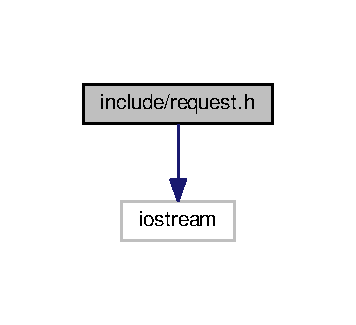
\includegraphics[width=171pt]{request_8h__incl}
\end{center}
\end{figure}
This graph shows which files directly or indirectly include this file\+:
\nopagebreak
\begin{figure}[H]
\begin{center}
\leavevmode
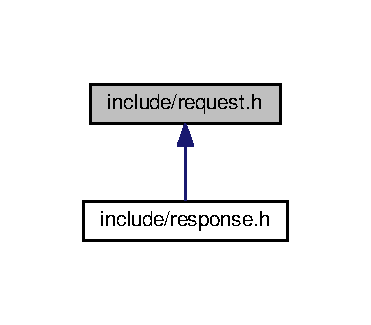
\includegraphics[width=178pt]{request_8h__dep__incl}
\end{center}
\end{figure}
\subsection*{Classes}
\begin{DoxyCompactItemize}
\item 
class \hyperlink{classRequest}{Request}
\begin{DoxyCompactList}\small\item\em defines a client request \end{DoxyCompactList}\end{DoxyCompactItemize}


\subsection{Detailed Description}
Wrapper for client request. 


\hypertarget{response_8h}{}\section{include/response.h File Reference}
\label{response_8h}\index{include/response.\+h@{include/response.\+h}}


Wrapper for server response.  


{\ttfamily \#include $<$request.\+h$>$}\\*
{\ttfamily \#include $<$actor.\+h$>$}\\*
{\ttfamily \#include $<$iostream$>$}\\*
{\ttfamily \#include $<$vector$>$}\\*
Include dependency graph for response.\+h\+:
\nopagebreak
\begin{figure}[H]
\begin{center}
\leavevmode
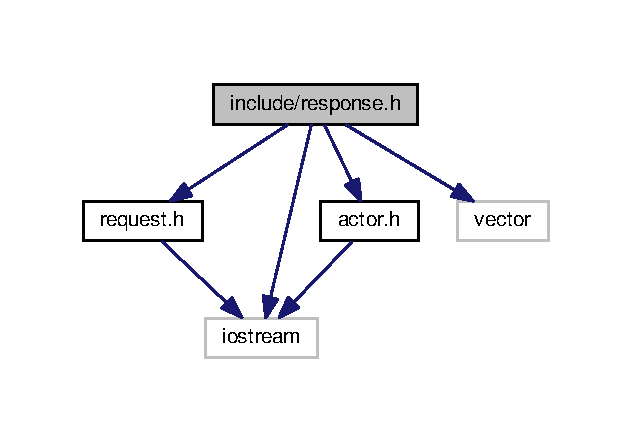
\includegraphics[width=304pt]{response_8h__incl}
\end{center}
\end{figure}
\subsection*{Classes}
\begin{DoxyCompactItemize}
\item 
class \hyperlink{classResponse}{Response}
\begin{DoxyCompactList}\small\item\em defines a server response \end{DoxyCompactList}\end{DoxyCompactItemize}


\subsection{Detailed Description}
Wrapper for server response. 


%--- End generated contents ---

% Index
\backmatter
\newpage
\phantomsection
\clearemptydoublepage
\addcontentsline{toc}{chapter}{Index}
\printindex

\end{document}
